\section{Epidemiological Time Series} \label{sec:epidemio}

This subsection presents a contextualization, contributions, datasets, and methodology adopted for application 1.

%%%%%%%%%%%%%%%%%%%%%%%%%%%%%%%%%%%%%%%%%%%%%%%%%%

\subsection{Contextualization and Contributions}

The \ac{COVID-19} is a viral infectious disease induced by \ac{SARS-CoV2}. According to the \ac{WHO}, most of the population will have mild to moderate respiratory illness and recover without requiring special treatment \cite{worldhealthorganizationwho2020Coronavirus}. However, several studies are being developed, and preliminary results indicated that people with underlying medical problems like cardiovascular disease, diabetes, chronic respiratory disease, obesity, and cancer are more likely to develop serious injuries \cite{bansal2020Cardiovascular,lai2020Severe,hussain2020COVID19,moujaess2020Cancer,abbas2020Mutual,su2020Renal}. Also, the \ac{COVID-19} can cause extensive, and multiple lung injuries \cite{guan2020Clinical}, thus compromising the respiratory system of patients. In this context, the demand for devices that assist in performing breathing-related movements has increased. 

Due to the severe damage caused by \ac{COVID-19}, according to \ac{WHO}, up to June 10th, 2020, more than 7.1 million people were already infected, as well as more than 400 thousand people worldwide have now died with the coronavirus. Indeed, considering the current scenario of the health system worldwide, overcrowding could be observed in some countries like Italy, Spain, and perhaps Brazil. In Brazil, it is believed that an average of 3,388 municipalities could have a significant deficit in hospital beds. Significantly, the debt is projected to occur in Brazilian North and Northeast regions, exceeding health care capacity due to the \ac{COVID-19} \cite{requia2020Risk}. 

In this respect, for forecasting cumulative cases of \ac{COVID-19}, the objective of this study is to explore and compare the predictive capacity of \ac{BRNN}, \ac{CUBIST}, \ac{KNN}, \ac{QRF}, and \ac{SVR} when are used stand-alone, and a hybrid framework composed by \ac{VMD} coupled with previously mentioned models. In this study were used as datasets the number of cumulative cases of \ac{COVID-19} from five Brazilian states (\ac{AM}, \ac{CE}, \ac{PE}, \ac{RJ}, and \ac{SP}), the first state from the north region, the second and third states from the northeast region, and the other two states from the southeast region. Also were considered five  American states (\ac{CA}, \ac{IL}, \ac{MA}, \ac{NJ}, and \ac{NY}). These states were chosen through the most significant number of new cases of \ac{COVID-19} up to April 28th, 2020.  

Forecasting horizons of the time series one, three, and six days ahead of cumulative \ac{COVID-19} cases are adopted to evaluate the forecasting efficiency of the different models. Additionally, previous \ac{COVID-19} cases and exogenous variables such as daily temperature (maximum and minimum) and precipitation are employed as inputs for each evaluated model. The output-of-sample forecasting accuracy of each model is compared by performance metrics such as the \ac{IP}, \ac{sMAPE}, and \ac{RRMSE}. Also, the importance of each input variable is presented for each mentioned country.

Forecasting models are impacted by the small dataset effect and the prediction of cases of \ac{COVID-19}, making a challenging task. The forecasting and preprocessing approaches are chosen because even though nonlinear and \ac{AI} models need large datasets to properly learn the data pattern, the use of exogenous variables (climate variables) and past values of the response variable overcomes this drawback.

\ac{VMD} decomposes a time series into its \ac{IMF}s adaptively and non-recursively, obtaining a set of sub-series with different features from low-frequency to high-frequency. Adopting \ac{VMD} with modes in conjunction with nonlinear machine learning prediction models is a robust framework to approach small datasets in forecasting tasks. In addition, \ac{BRNN} and \ac{SVR} approaches can handle small samples, making them attractive for this study. In consideration of the objectives of this application, the following \ac{RQ}s are defined:

\begin{enumerate}[wide=0pt, leftmargin=3em]
    \item[\textbf{RQ 1.1}] Can signal decomposition approaches enhance the performance of forecasting \ac{COVID-19} cumulative cases time series?
    
    \item[\textbf{RQ 2}] How does the use of exogenous features impact performance improvement when forecasting \ac{COVID-19} cumulative cases time series?
\end{enumerate}

To address the \ac{RQ}s of this application, the contributions can be summarized as follows: 

\begin{enumerate}[label=\alph*)]
    \item The first contribution is related to the proposal of two frameworks, non-decomposed and decomposed models, applied to forecast the new cumulative cases of \ac{COVID-19} in five Brazilian and American states. These evaluated models are expected to be used as the most accurate approaches to perform decision-making to structure the health system, avoid overcrowding in hospitals, and prevent new deaths. 
    
    \item The second contribution, we can highlight the use of a distinct set of \ac{AI} models based on machine learning approaches regarding learning structure, even as the recent effective preprocessing \ac{VMD} to forecasting the Brazilian and American \ac{COVID-19} new cumulative cases. The forecasting models \ac{BRNN}, \ac{CUBIST}, \ac{KNN}, \ac{QRF}, \ac{SVR}, and preprocessing \ac{VMD} method were chosen once they have reached success in several fields of regression and time series forecasting \cite{ribeiro2018Multiobjective,fernandez-delgado2019Extensive,zuo2020Decomposition,zhu2019Hybrid}; 
    
    \item Also, this study evaluates \ac{AI} models in a multi-day-ahead forecasting strategy coupled with exogenous climatic inputs. The range of the forecasting time horizon allows us to verify the effectiveness of the predicting models in different scenarios associated with information such as previous \ac{COVID-19} cumulative cases, temperature, and precipitation, allowing the models to achieve high forecasting accuracy. Finally, their results can help plan actions to improve the health system to contain the \ac{COVID-19} deaths.
\end{enumerate}

%%%%%%%%%%%%%%%%%%%%%%%%%%%%%%%%%%%%%%%%%%%%%%%%%%

\subsection{Dataset Description}

The collected dataset refers to the \ac{COVID-19} cumulative cases that occurred in five states of Brazil and \ac{USA} until April 20th, 2020. For the Brazilian context, the dataset was collected from an API (Application Program Interface) \cite{justen2020COVID19} that retrieves the daily information about \ac{COVID-19} cases from all 27 Brazilian State Health Offices, assembles and makes them publicly available. And for \ac{USA} context, the dataset was collected from ``\ac{COVID-19} Data Repository'' on Github provided by the \ac{CSSE} at Johns Hopkins University \cite{centerforsystemsscienceandengineeringcsse2020Novel}. The cumulative confirmed cases and deaths of each state, and the period from the first and last reports, are illustrated in Table~\ref{tab:reports}. 

% TABLE - Confirmed cases data
\begin{table}[htb!]
\small
\centering
\caption{Summary of COVID-19 cases by country and state}
\label{tab:reports}
\resizebox{\textwidth}{!}{%
\begin{tabular}{ccccccc}
\hline
\textbf{Country} &
  \textbf{State} &
  \textbf{Number of observed days} &
  \textbf{Fist reported} &
  \textbf{Last reported} &
  \textbf{Cumulative cases} &
  \textbf{Cumulative deaths} \\ \hline
\multirow{5}{*}{Brazil} & \ac{AM} & 47 & 13/03/2020 & 28/04/2020 & 4337   & 351   \\
                        & \ac{CE} & 44 & 16/03/2020 & 28/04/2020 & 6985   & 403   \\
                        & \ac{PE} & 48 & 12/03/2020 & 28/04/2020 & 5724   & 508   \\
                        & \ac{RJ} & 55 & 05/03/2020 & 28/04/2020 & 8504   & 738   \\
                        & \ac{SP} & 64 & 25/02/2020 & 28/04/2020 & 24041  & 2049  \\ \hline
\multirow{5}{*}{\ac{USA}}    & \ac{CA} & 94 & 26/01/2020 & 28/04/2020 & 46164  & 1864  \\
                        & \ac{IL} & 96 & 24/01/2020 & 28/04/2020 & 48102  & 2125  \\
                        & \ac{MA} & 87 & 01/02/2020 & 27/04/2020 & 56462  & 3003  \\
                        & \ac{NJ} & 55 & 05/03/2020 & 28/04/2020 & 113856 & 6442  \\
                        & \ac{NY} & 58 & 02/03/2020 & 28/04/2020 & 295106 & 22912 \\ \hline
\end{tabular}
}
\end{table}

The exogenous climatic variables were retrieved from the \ac{INMET} \cite{brazil2020Instituto} for data from Brazil, while the \ac{USA} climate dataset was taken into a count from the daily global historical climatology network that was retrieved from the \ac{NCEI} from the National Oceanic and Atmospheric Administration \cite{u.s.2020National}, by using \texttt{\{rnoaa\}} package \cite{chamberlain2020Rnoaa}. For each state, considering the daily available information, minimum and maximum temperature (\textit{ºC}) and precipitation (\textit{mm}) were selected as exogenous climatic inputs to each forecasting model applied in this study. The measurement period of each state is variable. This is because the record of the first case of the disease may differ from state to state. The summary of the climatic variables used is described in Table \ref{tab:climatic}.  

\begin{scriptsize}
\begin{center}
\begin{longtable}[htb!]{cclcccc}
\caption{Descriptive measures for climatic variables by country and state \label{tab:climatic}}\\
\hline
\textbf{Country} & \textbf{State} & \textbf{Variable} & \textbf{Minimum} & \textbf{Median} & \textbf{Mean} & \textbf{Maximum} \\ \hline \endfirsthead
  \multicolumn{7}{c}%
  {\tablename\ \thetable\ -- \textit{Continued from previous page}} \\ \hline
\textbf{Country} & \textbf{State} & \textbf{Variable} & \textbf{Minimum} & \textbf{Median} & \textbf{Mean} & \textbf{Maximum} \\ \hline \endhead \hline \multicolumn{7}{r}{\textit{Continued on next page}} \\
\endfoot
\hline
\endlastfoot

\multirow{15}{*}{Brazil} & \ac{AM} & Minimum temperature (\textit{ºC}) & 24.76 & 26.20 & 26.36 & 28.28 \\
 &  & Maximum temperature (\textit{ºC}) & 25.29 & 27.05 & 27.24 & 29.55 \\
 &  & Precipitation (\textit{mm}) & 0.00 & 0.11 & 0.33 & 2.40 \\ \cline{2-7}
 & \ac{CE} & Minimum temperature (\textit{ºC}) & 25.14 & 26.62 & 26.60 & 27.90 \\
 &  & Maximum temperature (\textit{ºC}) & 25.91 & 27.73 & 27.68 & 28.99 \\
 &  & Precipitation (\textit{mm}) & 0.00 & 0.12 & 0.25 & 1.31 \\ \cline{2-7}
 & \ac{PE} & Minimum temperature (\textit{ºC}) & 23.36 & 25.18 & 25.05 & 26.74 \\
 &  & Maximum temperature (\textit{ºC}) & 24.27 & 26.30 & 26.10 & 27.96 \\
 &  & Precipitation (\textit{mm}) & 0.00 & 0.14 & 0.23 & 1.33 \\ \cline{2-7}
 & \ac{RJ} & Minimum temperature (\textit{ºC}) & 19.07 & 21.23 & 21.57 & 25.33 \\
 &  & Maximum temperature (\textit{ºC}) & 19.69 & 22.16 & 22.56 & 26.49 \\
 &  & Precipitation (\textit{mm}) & 0.00 & 0.03 & 0.13 & 1.32 \\ \cline{2-7}
 & \ac{SP} & Minimum temperature (\textit{ºC}) & 17.60 & 19.99 & 20.09 & 23.40 \\
 &  & Maximum temperature (\textit{ºC}) & 18.76 & 21.11 & 21.37 & 25.03 \\
 &  & Precipitation (\textit{mm}) & 0.00 & 0.00 & 0.12 & 1.19 \\ \hline
\multirow{15}{*}{\ac{USA}} & {\ac{CA}} & Minimum temperature (\textit{ºC}) & -1.76 & 4.90 & 4.91 & 11.92 \\
 &  & Maximum temperature (\textit{ºC}) & 10.60 & 18.33 & 18.54 & 28.59 \\
 &  & Precipitation (\textit{mm}) & 0.01 & 4.66 & 20.98 & 162.67 \\ \cline{2-7}
 & \ac{IL} & Minimum temperature (\textit{ºC}) & -19.42 & -0.42 & -0.75 & 14.63 \\
 &  & Maximum temperature (\textit{ºC}) & -6.39 & 8.40 & 8.99 & 26.06 \\
 &  & Precipitation (\textit{mm}) & 0.00 & 4.29 & 23.30 & 196.47 \\ \cline{2-7}
 & \ac{MA} & Minimum temperature (\textit{ºC}) & -14.75 & -0.86 & -1.76 & 5.39 \\
 &  & Maximum temperature (\textit{ºC}) & -2.77 & 8.32 & 8.16 & 18.70 \\
 &  & Precipitation (\textit{mm}) & 0.00 & 6.84 & 34.66 & 320.86 \\ \cline{2-7}
 & \ac{NJ} & Minimum temperature (\textit{ºC}) & -11.80 & 1.60 & 0.96 & 7.27 \\
 &  & Maximum temperature (\textit{ºC}) & 0.54 & 10.78 & 11.22 & 22.02 \\
 &  & Precipitation (\textit{mm}) & 0.00 & 5.44 & 31.53 & 274.04 \\ \cline{2-7}
 & \ac{NY} & Minimum temperature (\textit{ºC}) & -20.48 & -2.61 & -3.75 & 4.60 \\
 &  & Maximum temperature (\textit{ºC}) & -7.98 & 5.62 & 6.23 & 17.88 \\
 &  & Precipitation (\textit{mm}) & 0.00 & 9.94 & 27.61 & 167.94 \\ \hline
\end{longtable}
\end{center}
\end{scriptsize}

The heatmap of the cumulative confirmed cases from Brazil and \ac{USA} in each of the five states analyzed are presented in Figure~\ref{fig:heatmap}. In that figure, the states with the highest number of \ac{COVID-19} cumulative cases are \ac{SP} and \ac{NY}, respectively, in Brazil and \ac{USA}, the states with the highest demographic index in both countries.

% FIGURE - Heatmap
\begin{figure}[htb!]
    \centering
    % \subfloat[Brazil \label{subfig:heatmap_BRA}]{
    %     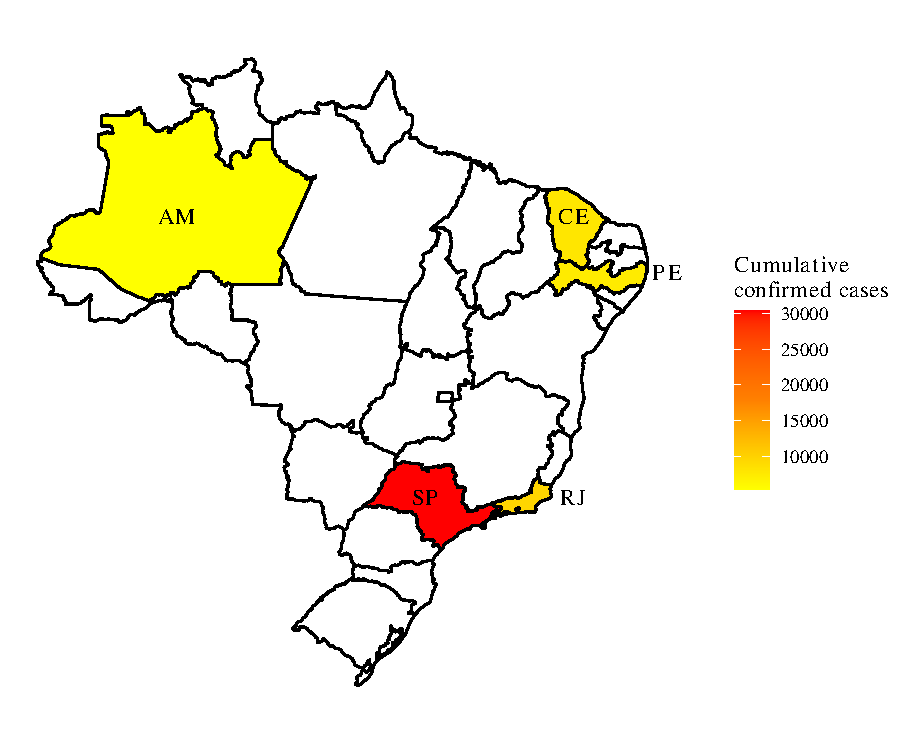
\includegraphics[width=.385\linewidth]{Media/cs1_heatmap_bra.pdf}
    % }
    % %
    % \subfloat[\ac{USA} \label{subfig:heatmap_USA}]{
    %     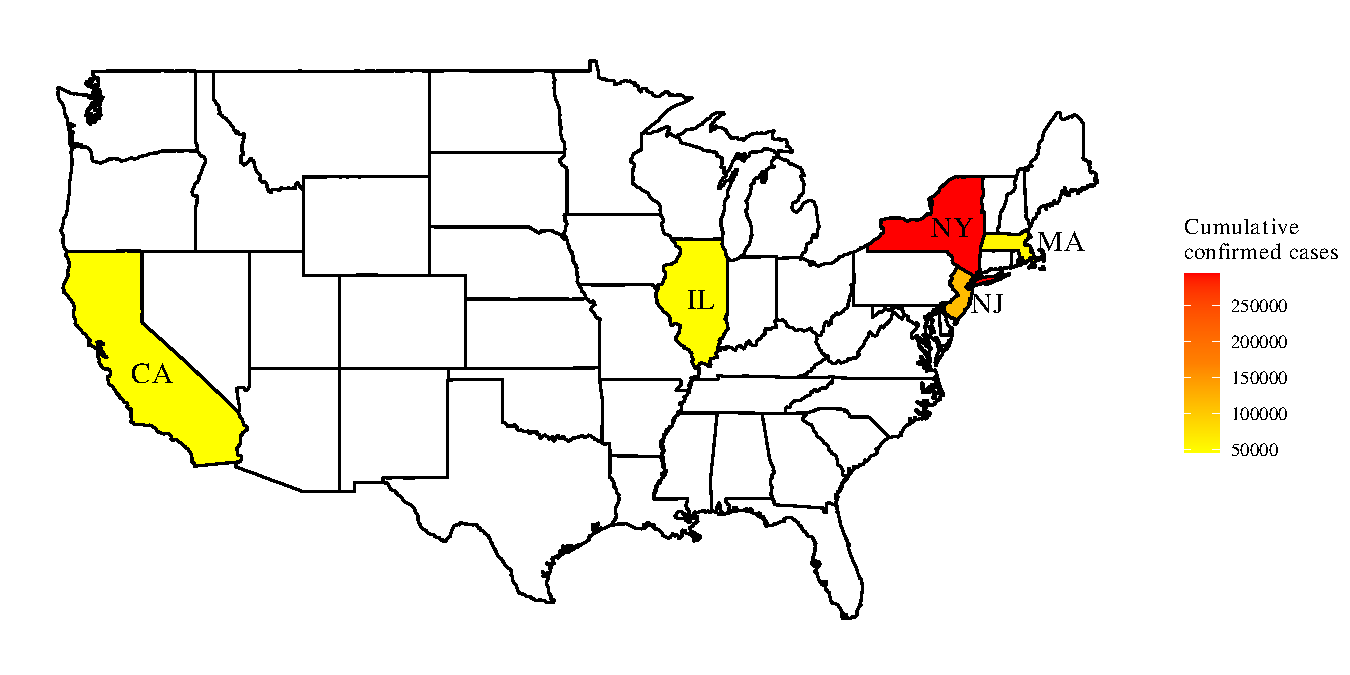
\includegraphics[width=.575\linewidth]{Media/cs1_heatmap_usa.pdf}
    % }
    \subfloat[Brazil \label{subfig:heatmap_BRA}]{
        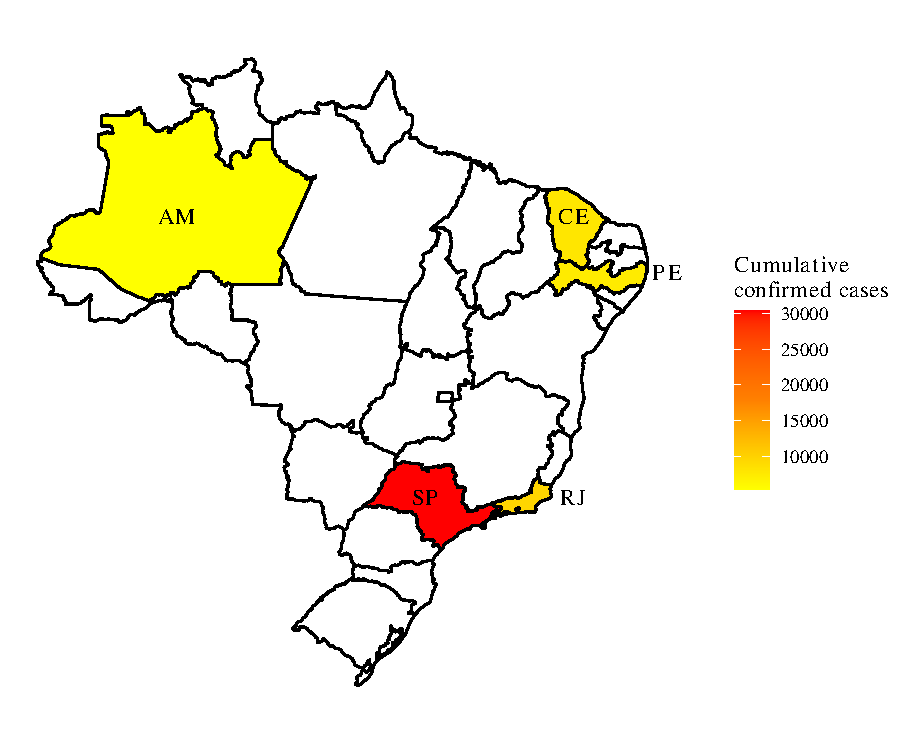
\includegraphics[width=.7\linewidth]{Media/cs1_heatmap_bra.pdf}
    }
    
    \subfloat[\ac{USA} \label{subfig:heatmap_USA}]{
        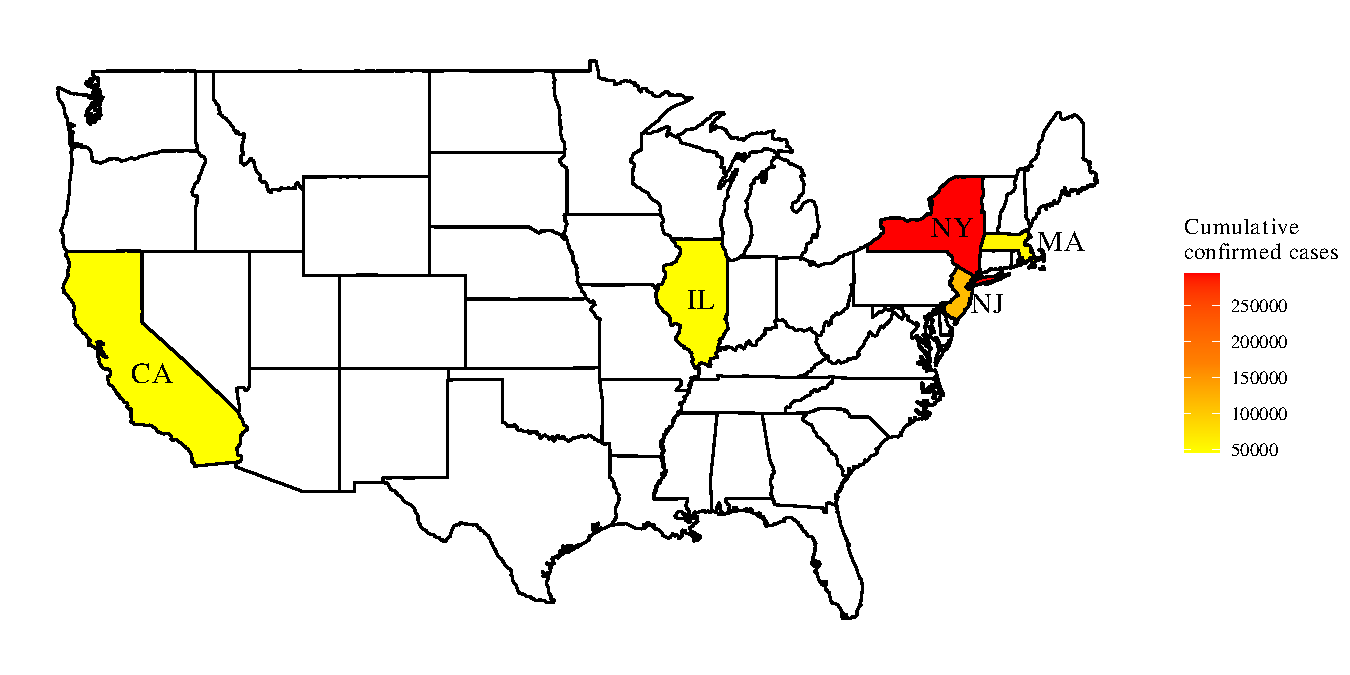
\includegraphics[width=.9\linewidth]{Media/cs1_heatmap_usa.pdf}
    }
    \caption{Heatmap of the cumulative confirmed cases to five states from Brazil and USA.}
    \label{fig:heatmap}
    \source{\citeonline{dasilva2020Forecasting}}
\end{figure}

%%%%%%%%%%%%%%%%%%%%%%%%%%%%%%%%%%%%%%%%%%%%%%%%%%

\subsection{Proposed Forecasting Framework}

This section describes the main steps in the data analysis adopted by \ac{BRNN}, \ac{CUBIST}, \ac{KNN}, \ac{QRF}, \ac{SVR}, and \ac{VMD} based models. 

\begin{enumerate}[start=1,label={\textbf{Step \arabic*:}},wide = 0pt, leftmargin = 3em]
\item \label{step1} First, the dataset output variables are decomposed into five \ac{IMF}s by performing \ac{VMD}. The lag equal 2 was chosen by grid-search, applied on the \ac{IMF}s creating four inputs from the lags, and applied on the exogenous inputs. Further, the new data is split into training and test sets. The test set consists of the last six observations, and the remaining samples define the training set. In the training state, leave one-out-cross-validation with time slice was adopted, such as developed by \citeonline{ribeiro2020Ensemble}.

\item \label{step2} Each \ac{IMF} is trained with each model presented before using the time-slice validation approach. Next, a simple summation-grouping model reconstructed the \ac{IMF} predictions. In other words, the \ac{IMF} is trained by the same model and is summed. Then, five predictions outputs were generated named \ac{VMD}--\ac{BRNN}, \ac{VMD}--\ac{CUBIST}, \ac{VMD}--\ac{KNN}, \ac{VMD}--\ac{QRF}, and \ac{VMD}--\ac{SVR}.

\item \label{step3} A recursive strategy is employed to develop multi-days-ahead \ac{COVID-19} cases forecasting \cite{ribeiro2020Shortterm}. Regarding this, one model is fitted for one-day-ahead forecasting. Then the recursive strategy uses this forecasting result as an input for the same model to forecast the next step, continuing until the desirable forecasting horizon. In this study, the aim is to obtain the cases up to $H$ next days, especially up to \ac{ODA}, \ac{TDA}, and \ac{SDA}, respectively. The following structures are considered as

\begin{equation}
    \hat{y}_{(t+h)} =
    \begin{cases}
    \hat{f}\left\{y_{(t+h-1)}, \,y_{(t+h-2)},\,\mathbf{X}_{(t+h-1)}\right\} & \text{if } h = 1, \\
    \hat{f}\left\{\hat{y}_{(t+h-1)},\,\hat{y}_{(t+h-2)},\, \mathbf{X}_{(t+h-3)}\right\} & \text{if } h = 3, \\
    \hat{f}\left\{\hat{y}_{(t+h-1)},\, \hat{y}_{(t+h-2)},\, \mathbf{X}_{(t+h-6)}\right\} & \text{if } h = 6, \\
    \end{cases}
\end{equation}
where $\hat{f}$ is a function that maps the cumulative \ac{COVID-19} cases, $\hat{y}(t+h)$ is the forecast of cumulative cases in horizon $h=$1, 3 and 6, $y(t+h-1)$, ${y}(t+h-2)$ are the previous observed, $\hat{y}(t+h-1)$, $\hat{y}(t+h-2)$ are the predicted cumulative cases, $\mathbf{X}(t+h-n_x)$ is the exogenous inputs vector at the maximum lag of inputs ($n_x = 1$ if $h = 1$, $n_x = 3$ if $h = 3$, and $n_x = 6$ if $h = 6$). All hyperparameters employed in this study are presented in Tables \ref{tab:hyper1} and \ref{tab:hyper2} in Appendix~\ref{app:cs1_appendixA}.  

\item To evaluate the effectiveness of adopted models, from obtained forecasts out-of-sample (test set), \ac{IP}, \ac{sMAPE}, and \ac{RRMSE} criteria are computed. Figure \ref{fig:flowchart} presents the proposed forecasting framework.

% FIGURE - Diagram
\begin{figure}[htb!]
    \centering
    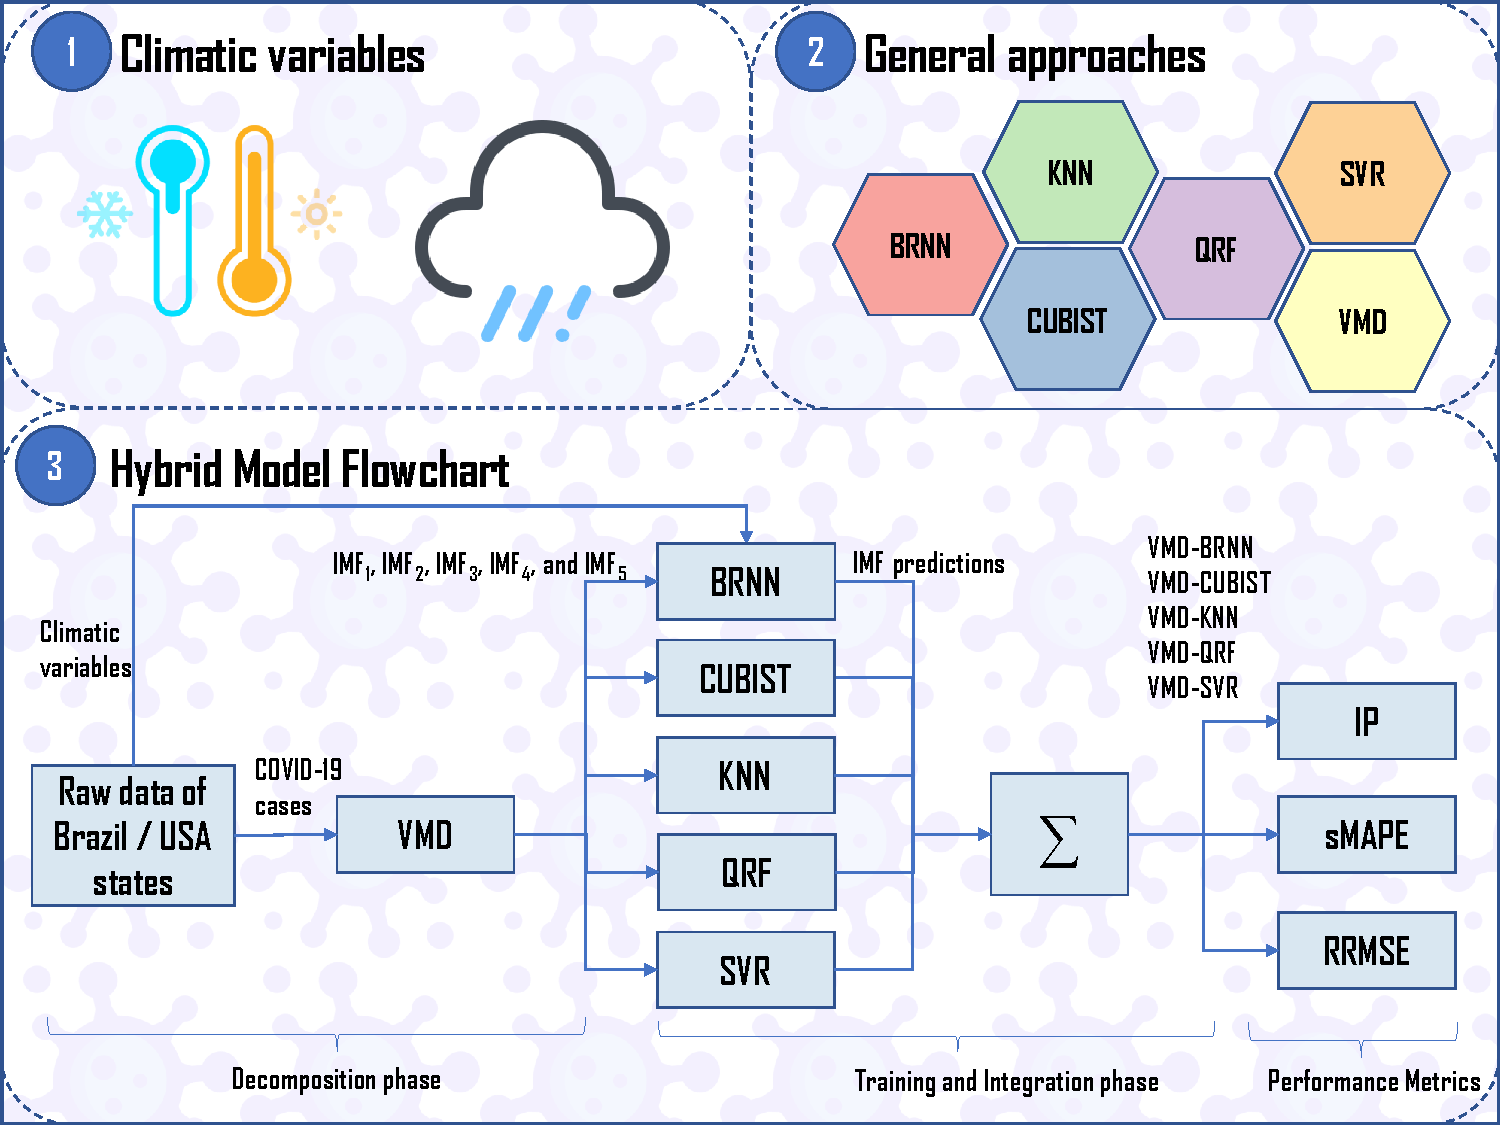
\includegraphics[width=0.9\linewidth]{Media/cs1_framework.pdf}
    \caption{Proposed forecasting framework for Application 1}
    \label{fig:flowchart}
    \source{\citeonline{dasilva2020Forecasting}}
\end{figure}

\end{enumerate}